\chapter{Annexes}

\section{Hyperparameter Optimization Contours}\label{sec:annex-contours}

This annex presents the hyperparameter optimization contour plots for
the three different labeling rates (LR) experimented in this work:
1.0, 0.5, and 0.3. The optimization process was performed using
Bayesian optimization with the \textit{Optuna} framework, and the results are
visualized through contour plots showing the relationship between
different hyperparameter pairs and their impact on model performance.

\subsection{Labeling Rate 1.0}

\subsubsection{Missing Labels Penalty Hyperparameters}

\begin{figure}[H]
  \centering
  \begin{subfigure}[b]{0.48\textwidth}
    \centering
    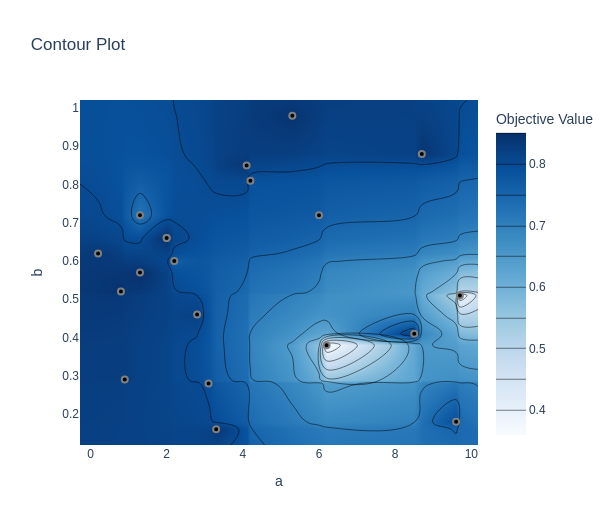
\includegraphics[width=\textwidth]{Annex/contours/lr1/features_a_b.png}
    \caption{Features space: $\alpha_{\lambda}$ vs $\beta$}
    \label{fig:lr1_features_ab}
  \end{subfigure}
  \hfill
  \begin{subfigure}[b]{0.48\textwidth}
    \centering
    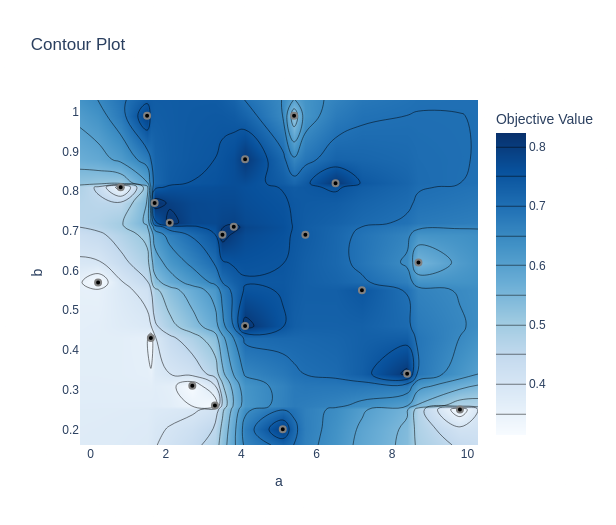
\includegraphics[width=\textwidth]{Annex/contours/lr1/pixel_a_b.png}
    \caption{Pixel space: $\alpha_{\lambda}$ vs $\beta$}
    \label{fig:lr1_pixel_ab}
  \end{subfigure}
  \vspace{0.5cm}
  \begin{subfigure}[b]{0.48\textwidth}
    \centering
    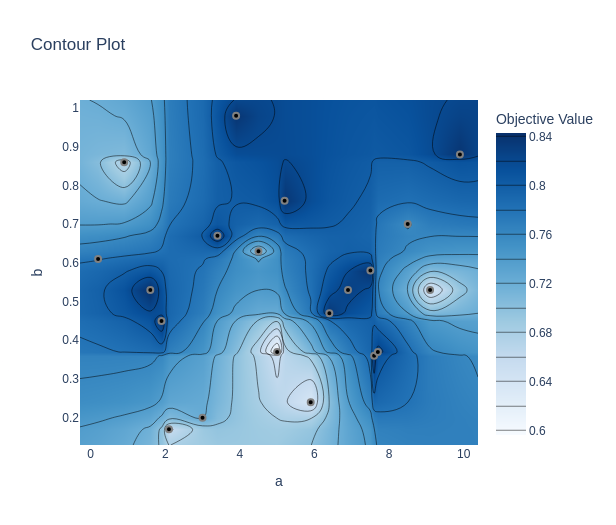
\includegraphics[width=\textwidth]{Annex/contours/lr1/scalar_a_b.png}
    \caption{Scalar space: $\alpha_{\lambda}$ vs $\beta$}
    \label{fig:lr1_scalar_ab}
  \end{subfigure}
  \caption{Hyperparameter optimization contours for labeling rate 1.0
    showing the relationship between $\alpha_{\lambda}$ and $\beta$
  parameters across different feature spaces.}
  \label{fig:lr1_ab_contours}
\end{figure}

\subsubsection{Other Hyperparameters}

\begin{figure}[H]
  \centering
  \begin{subfigure}[b]{0.48\textwidth}
    \centering
    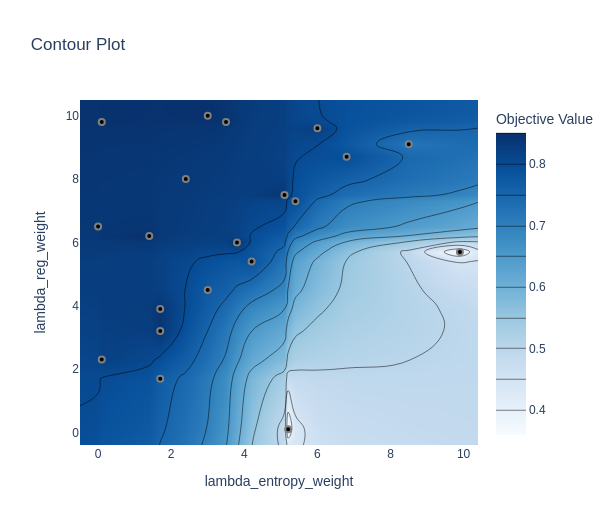
\includegraphics[width=\textwidth]{Annex/contours/lr1/features_others.png}
    \caption{Features space: Other hyperparameters}
    \label{fig:lr1_features_others}
  \end{subfigure}
  \hfill
  \begin{subfigure}[b]{0.48\textwidth}
    \centering
    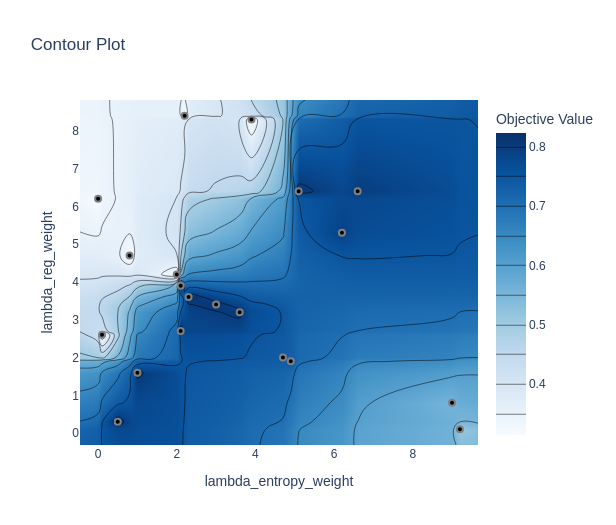
\includegraphics[width=\textwidth]{Annex/contours/lr1/pixel_others.png}
    \caption{Pixel space: Other hyperparameters}
    \label{fig:lr1_pixel_others}
  \end{subfigure}
  \vspace{0.5cm}
  \begin{subfigure}[b]{0.48\textwidth}
    \centering
    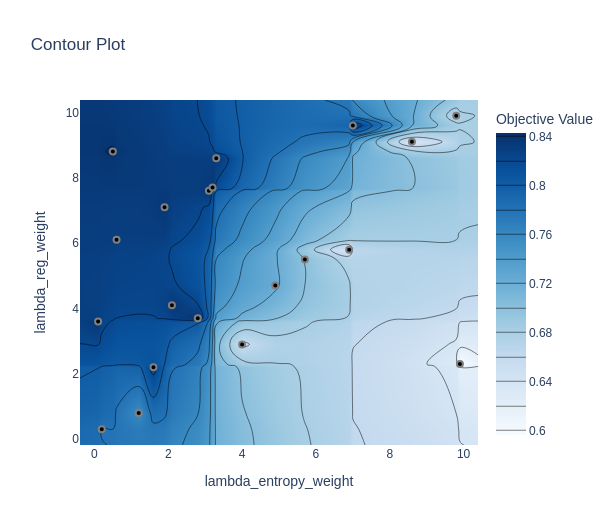
\includegraphics[width=\textwidth]{Annex/contours/lr1/scalar_others.png}
    \caption{Scalar space: Other hyperparameters}
    \label{fig:lr1_scalar_others}
  \end{subfigure}
  \caption{Hyperparameter optimization contours for labeling rate 1.0
    showing the relationship between other hyperparameters (centroid
  and entropy) across different feature spaces.}
  \label{fig:lr1_others_contours}
\end{figure}

\subsection{Labeling Rate 0.5}

\subsubsection{Missing Labels Penalty Hyperparameters}

\begin{figure}[H]
  \centering
  \begin{subfigure}[b]{0.48\textwidth}
    \centering
    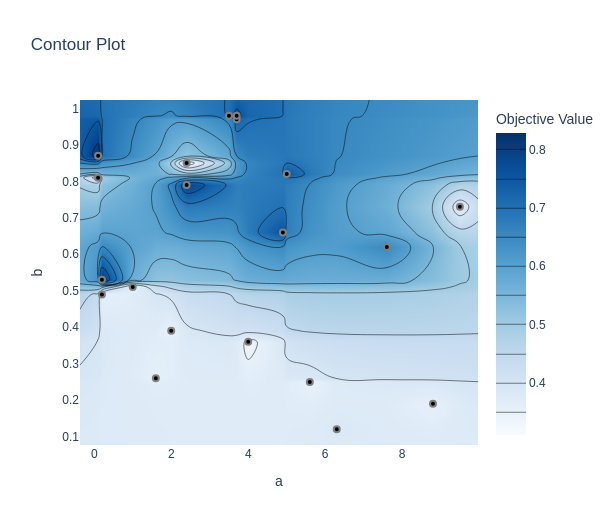
\includegraphics[width=\textwidth]{Annex/contours/lr0_5/features_a_b.png}
    \caption{Features space: $\alpha_{\lambda}$ vs $\beta$}
    \label{fig:lr05_features_ab}
  \end{subfigure}
  \hfill
  \begin{subfigure}[b]{0.48\textwidth}
    \centering
    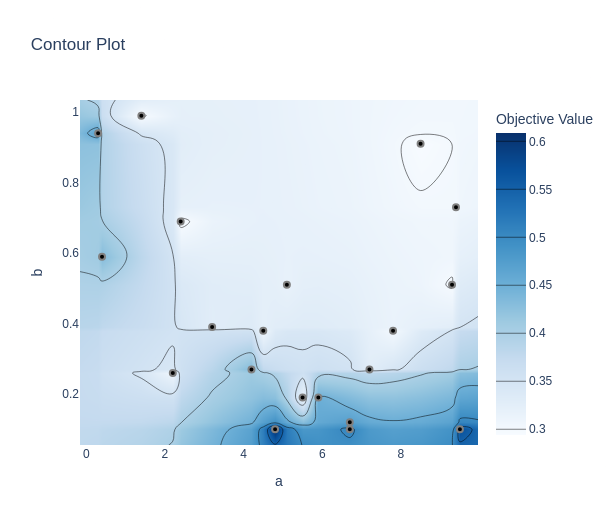
\includegraphics[width=\textwidth]{Annex/contours/lr0_5/pixel_a_b.png}
    \caption{Pixel space: $\alpha_{\lambda}$ vs $\beta$}
    \label{fig:lr05_pixel_ab}
  \end{subfigure}
  \vspace{0.5cm}
  \begin{subfigure}[b]{0.48\textwidth}
    \centering
    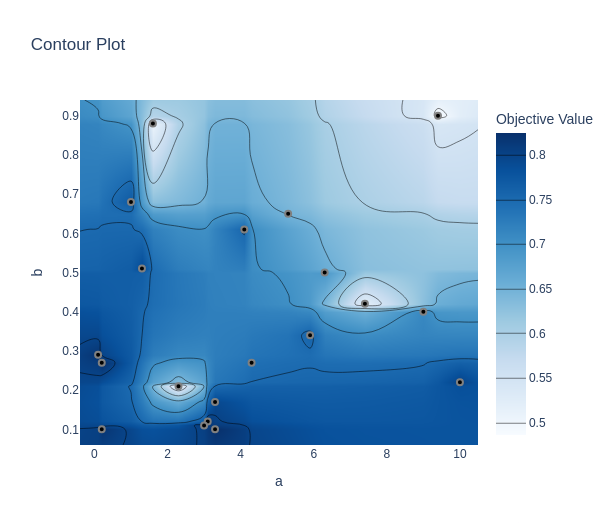
\includegraphics[width=\textwidth]{Annex/contours/lr0_5/scalar_a_b.png}
    \caption{Scalar space: $\alpha_{\lambda}$ vs $\beta$}
    \label{fig:lr05_scalar_ab}
  \end{subfigure}
  \caption{Hyperparameter optimization contours for labeling rate 0.5
    showing the relationship between $\alpha_{\lambda}$ and $\beta$
  parameters across different feature spaces.}
  \label{fig:lr05_ab_contours}
\end{figure}

\subsubsection{Other Hyperparameters}

\begin{figure}[H]
  \centering
  \begin{subfigure}[b]{0.48\textwidth}
    \centering
    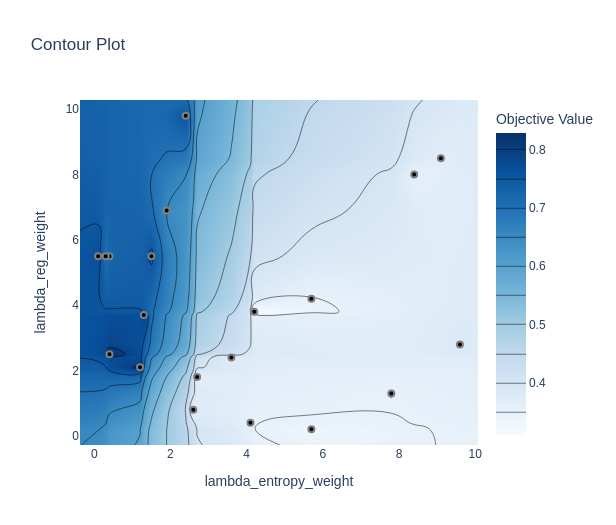
\includegraphics[width=\textwidth]{Annex/contours/lr0_5/features_others.png}
    \caption{Features space: Other hyperparameters}
    \label{fig:lr05_features_others}
  \end{subfigure}
  \hfill
  \begin{subfigure}[b]{0.48\textwidth}
    \centering
    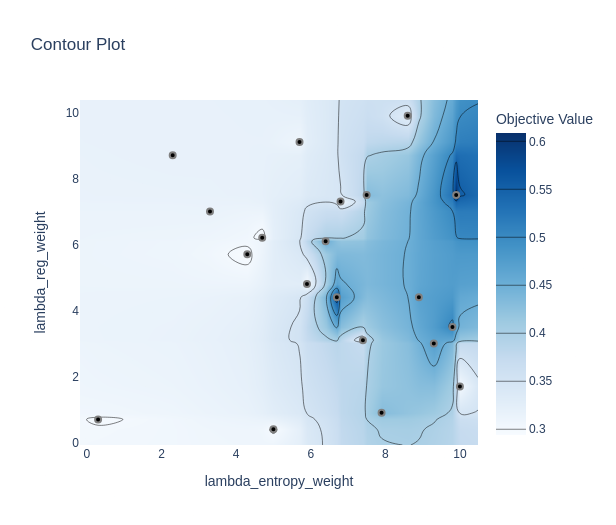
\includegraphics[width=\textwidth]{Annex/contours/lr0_5/pixel_others.png}
    \caption{Pixel space: Other hyperparameters}
    \label{fig:lr05_pixel_others}
  \end{subfigure}
  \vspace{0.5cm}
  \begin{subfigure}[b]{0.48\textwidth}
    \centering
    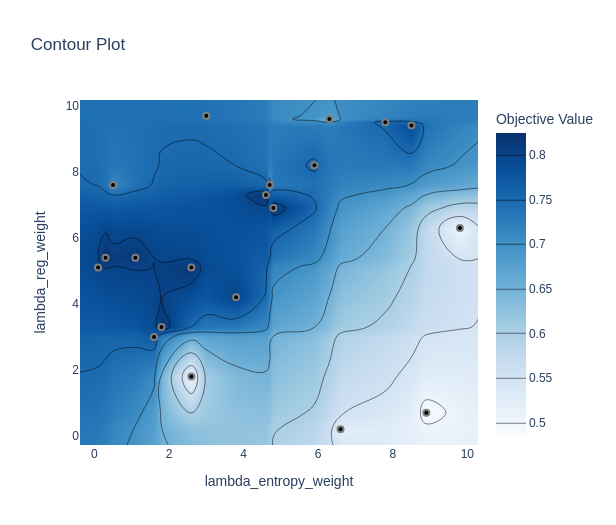
\includegraphics[width=\textwidth]{Annex/contours/lr0_5/scalar_others.png}
    \caption{Scalar space: Other hyperparameters}
    \label{fig:lr05_scalar_others}
  \end{subfigure}
  \caption{Hyperparameter optimization contours for labeling rate 0.5
    showing the relationship between other hyperparameters (centroid
  and entropy) across different feature spaces.}
  \label{fig:lr05_others_contours}
\end{figure}

\subsection{Labeling Rate 0.3}

\subsubsection{Missing Labels Penalty Hyperparameters}

\begin{figure}[H]
  \centering
  \begin{subfigure}[b]{0.48\textwidth}
    \centering
    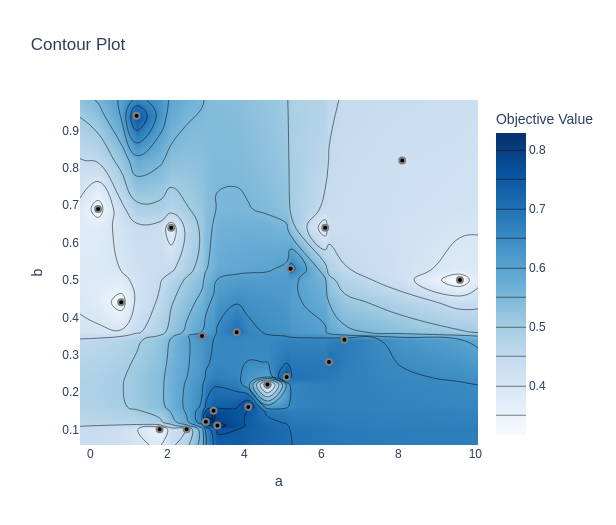
\includegraphics[width=\textwidth]{Annex/contours/lr0_3/features_a_b.png}
    \caption{Features space: $\alpha_{\lambda}$ vs $\beta$}
    \label{fig:lr03_features_ab}
  \end{subfigure}
  \hfill
  \begin{subfigure}[b]{0.48\textwidth}
    \centering
    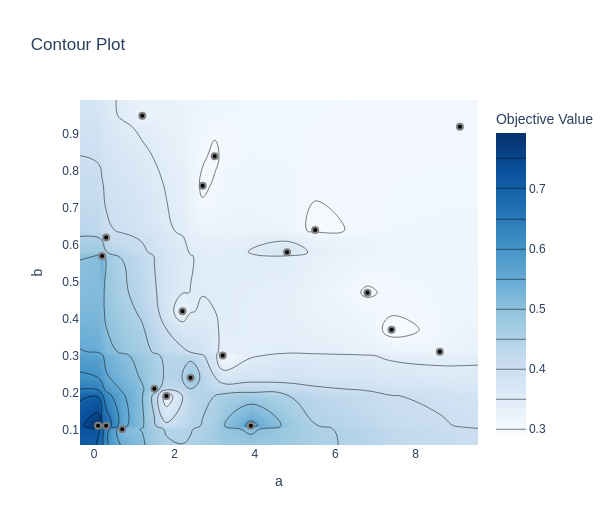
\includegraphics[width=\textwidth]{Annex/contours/lr0_3/pixel_a_b.png}
    \caption{Pixel space: $\alpha_{\lambda}$ vs $\beta$}
    \label{fig:lr03_pixel_ab}
  \end{subfigure}
  \vspace{0.5cm}
  \begin{subfigure}[b]{0.48\textwidth}
    \centering
    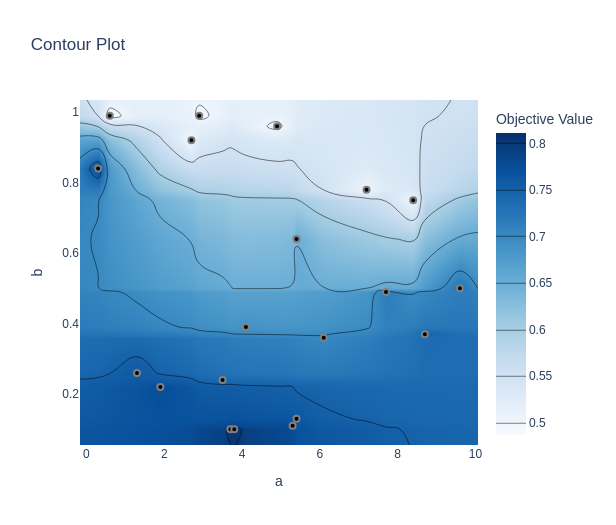
\includegraphics[width=\textwidth]{Annex/contours/lr0_3/scalar_a_b.png}
    \caption{Scalar space: $\alpha_{\lambda}$ vs $\beta$}
    \label{fig:lr03_scalar_ab}
  \end{subfigure}
  \caption{Hyperparameter optimization contours for labeling rate 0.3
    showing the relationship between $\alpha_{\lambda}$ and $\beta$
  parameters across different feature spaces.}
  \label{fig:lr03_ab_contours}
\end{figure}

\subsubsection{Other Hyperparameters}

\begin{figure}[H]
  \centering
  \begin{subfigure}[b]{0.48\textwidth}
    \centering
    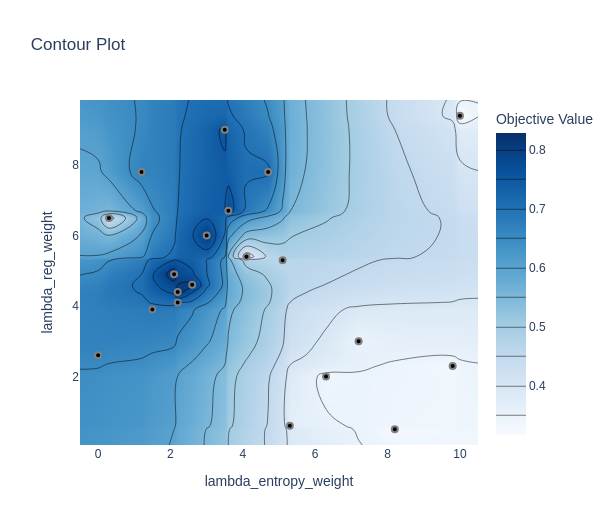
\includegraphics[width=\textwidth]{Annex/contours/lr0_3/features_others.png}
    \caption{Features space: Other hyperparameters}
    \label{fig:lr03_features_others}
  \end{subfigure}
  \hfill
  \begin{subfigure}[b]{0.48\textwidth}
    \centering
    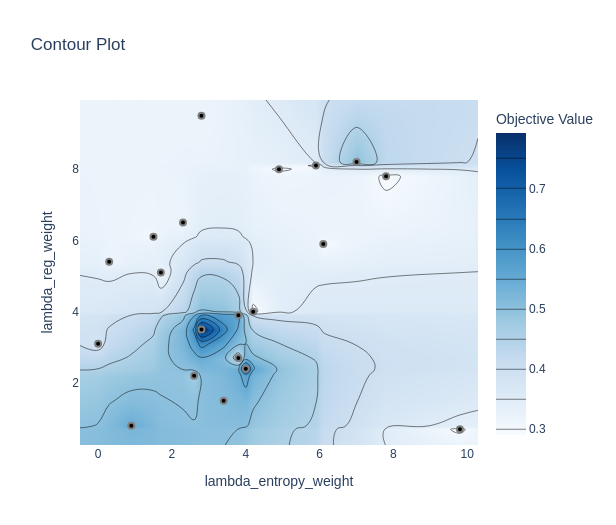
\includegraphics[width=\textwidth]{Annex/contours/lr0_3/pixel_others.png}
    \caption{Pixel space: Other hyperparameters}
    \label{fig:lr03_pixel_others}
  \end{subfigure}
  \vspace{0.5cm}
  \begin{subfigure}[b]{0.48\textwidth}
    \centering
    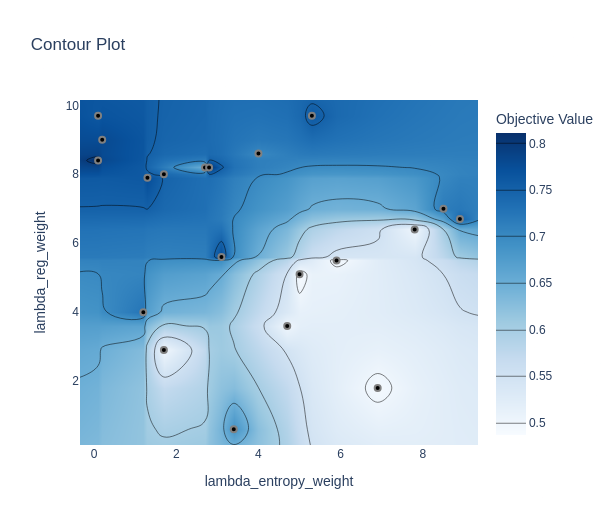
\includegraphics[width=\textwidth]{Annex/contours/lr0_3/scalar_others.png}
    \caption{Scalar space: Other hyperparameters}
    \label{fig:lr03_scalar_others}
  \end{subfigure}
  \caption{Hyperparameter optimization contours for labeling rate 0.3
    showing the relationship between other hyperparameters (centroid
  and entropy) across different feature spaces.}
  \label{fig:lr03_others_contours}
\end{figure}

\section{Analysis of Hyperparameter Optimization Results}

The hyperparameter importance analysis reveals distinct patterns
across different labeling rates and feature spaces, with
$\alpha_{\text{entropy}}$ emerging as the most critical
hyperparameter overall (average importance: 0.464), followed by
$\beta$ (0.230), $\alpha_{\text{centroid}}$ (0.172), and
$\alpha_{\lambda}$ (0.133). However, the importance distribution
varies dramatically across feature spaces, indicating that
hyperparameter optimization strategies must be tailored to the
specific representation space being used.

In the features space, $\alpha_{\text{entropy}}$ exhibits extreme
dominance, reaching importance values of 0.8458 at LR 0.3 and peaking
at 0.9586 at LR 0.5, while all other hyperparameters remain below
0.05 importance. This suggests that entropy-based regularization is
particularly crucial when working with high-dimensional feature
representations, where the entropy term effectively guides the
learning process. Conversely, the pixel space shows a more moderate
distribution with $\beta$ being the most important hyperparameter
(0.4313 at LR 0.3, 0.4757 at LR 0.5), indicating that the missing
labels penalty weight is more critical when operating directly on
pixel-level representations. The scalar space demonstrates the most
balanced importance distribution, with $\alpha_{\text{entropy}}$
leading at 0.8168 for LR 1.0, suggesting that scalar representations
benefit from a more nuanced approach to hyperparameter selection.

The learning rate dependencies reveal that as the labeling rate
decreases from 1.0 to 0.3, the importance patterns become more
pronounced and space-specific. At LR 0.3, the features space is
dominated by $\alpha_{\text{entropy}}$ (0.8458) while the pixel space
relies heavily on $\beta$ (0.4313). At LR 0.5,
$\alpha_{\text{entropy}}$ reaches its peak importance in the features
space (0.9586), while $\beta$ maintains its importance in the pixel
space (0.4757). By LR 1.0, the distribution becomes more balanced,
with $\alpha_{\text{entropy}}$ leading in the scalar space (0.8168)
and $\alpha_{\text{centroid}}$ showing increased importance in the
features space (0.2134).

The statistical correlation analysis, presented in
Table~\ref{tab:hyperparameter_correlations}, reveals several
significant patterns that further illuminate the relationship between
hyperparameters and learning rates across different feature spaces.
These correlations demonstrate that hyperparameter importance is not
only space-dependent but also exhibits predictable trends with
respect to the learning rate, supporting the development of adaptive
hyperparameter optimization strategies.

\begin{table}[H]
  \centering
  \caption{Correlation coefficients between hyperparameters and
  learning rate across different feature spaces}
  \label{tab:hyperparameter_correlations}
  \begin{tabular}{lccc}
    \toprule
    \textbf{Hyperparameter} & \textbf{Pixel Space} & \textbf{Scalar
    Space} & \textbf{Features Space} \\
    \midrule
    $\alpha_{\text{entropy}}$ & $r=0.361$, $p=1.225$ & $r=1.000$,
    $p=2.000$ & $r=-0.858$, $p=-1.334$ \\
    $\alpha_{\text{centroid}}$ & $r=0.211$, $p=1.568$ & $r=-0.660$,
    $p=0.244$ & $r=0.923$, $p=-2.785$ \\
    $\alpha_{\lambda}$ & $r=0.609$, $p=0.466$ & $r=0.270$, $p=1.439$
    & $r=0.812$, $p=-0.781$ \\
    $\beta$ & $r=-0.911$, $p=-2.421$ & $r=-0.766$, $p=-0.382$ &
    $r=-0.384$, $p=1.167$ \\
    \bottomrule
  \end{tabular}
\end{table}

These quantitative findings demonstrate that hyperparameter
importance is highly dependent on both the feature space and labeling
rate, supporting the need for space-specific and rate-specific
hyperparameter optimization strategies. The strong correlations
observed, particularly the perfect positive correlation between
$\alpha_{\text{entropy}}$ and learning rate in scalar space
($r=1.000$) and the strong negative correlation between $\beta$ and
learning rate in pixel space ($r=-0.911$), provide clear guidance for
developing adaptive hyperparameter selection algorithms that can
automatically adjust to different experimental conditions.
